\documentclass{article}

\usepackage{fancyhdr}
\usepackage{extramarks}
\usepackage{amsmath}
\usepackage{amsthm}
\usepackage{amsfonts}
\usepackage{tikz}
\usepackage[plain]{algorithm}
\usepackage{algpseudocode}
\usepackage{enumerate}
\usepackage{tikz}
\usepackage{xifthen}
\usepackage{xparse}
\usepackage{amsmath, amssymb}
\usepackage{lipsum}

\usetikzlibrary{automata,positioning}

%
% Basic Document Settings
%  

\topmargin=-0.45in
\evensidemargin=0in
\oddsidemargin=0in
\textwidth=6.5in
\textheight=9.0in
\headsep=0.25in

\linespread{1.1}

\pagestyle{fancy}
\lhead{\hmwkAuthorName}
\chead{\hmwkClass: \hmwkTitle}
\rhead{\firstxmark}
\lfoot{\lastxmark}
\cfoot{\thepage}

\renewcommand\headrulewidth{0.4pt}
\renewcommand\footrulewidth{0.4pt}

\setlength\parindent{0pt}

%
% Create Problem Sections
%

\newcommand{\enterProblemHeader}[1]{
    \nobreak\extramarks{}{Problem \arabic{#1} continued on next page\ldots}\nobreak{}
    \nobreak\extramarks{Problem \arabic{#1} (continued)}{Problem \arabic{#1} continued on next page\ldots}\nobreak{}
}

\newcommand{\exitProblemHeader}[1]{
    \nobreak\extramarks{Problem \arabic{#1} (continued)}{Problem \arabic{#1} continued on next page\ldots}\nobreak{}
    \stepcounter{#1}
    \nobreak\extramarks{Problem \arabic{#1}}{}\nobreak{}
}

\newcommand*\circled[1]{\tikz[baseline=(char.base)]{
		\node[shape=circle,draw,inner sep=2pt] (char) {#1};}}


\setcounter{secnumdepth}{0}
\newcounter{partCounter}
\newcounter{homeworkProblemCounter}
\setcounter{homeworkProblemCounter}{1}
\nobreak\extramarks{Problem \arabic{homeworkProblemCounter}}{}\nobreak{}

%
% Homework Problem Environment
%
% This environment takes an optional argument. When given, it will adjust the
% problem counter. This is useful for when the problems given for your
% assignment aren't sequential. See the last 3 problems of this template for an
% example.
%

\NewDocumentEnvironment{homeworkProblem}{s m}{
    \IfBooleanT{#1}{\newpage}
    \section{Problem \arabic{homeworkProblemCounter} {\small (#2)}}
    \setcounter{partCounter}{1}
    \enterProblemHeader{homeworkProblemCounter}

}{
    \exitProblemHeader{homeworkProblemCounter}
}

%
% Homework Details
%   - Title
%   - Due date
%   - Class
%   - Instructor
%   - Class number
%   - Name
%   - Student ID

\newcommand{\hmwkTitle}{Homework\ \#6}
\newcommand{\hmwkDueDate}{September 18, 2022}
\newcommand{\hmwkClass}{Probability and Mathematical Statistics}
\newcommand{\hmwkClassInstructor}{Professor Ziyu Shao}

\newcommand{\hmwkClassID}{\circled{0}}

\newcommand{\hmwkAuthorName}{Zhu Zhelin}
\newcommand{\hmwkAuthorID}{2021533077}

%
% Title Page
%

\title{
    \vspace{2in}
    \textmd{\textbf{\hmwkClass:\\  \hmwkTitle}}\\
    \normalsize\vspace{0.1in}\small{Due\ on\ \hmwkDueDate\ at 11:59am}\\
   \vspace{2in}\Huge{\hmwkClassID}\\   
   \vspace{2in}
}

\author{
	Name: \textbf{\hmwkAuthorName} \\
	Student ID: \hmwkAuthorID}
\date{}


\renewcommand{\part}[1]{\textbf{\large Part (\alph{partCounter})}\stepcounter{partCounter}\\}

%
% Various Helper Commands
%

% Useful for algorithms
\newcommand{\alg}[1]{\textsc{\bfseries \footnotesize #1}}
% For derivatives
\newcommand{\deriv}[1]{\frac{\mathrm{d}}{\mathrm{d}x} (#1)}
% For partial derivatives
\newcommand{\pderiv}[2]{\frac{\partial}{\partial #1} (#2)}
% Integral dx
\newcommand{\dx}{\mathrm{d}x}
% Alias for the Solution section header
\newcommand{\solution}{\textbf{\Large Solution}}
% Probability commands: Expectation, Variance, Covariance, Bias
\newcommand{\E}{\mathrm{E}}
\newcommand{\Var}{\mathrm{Var}}
\newcommand{\Cov}{\mathrm{Cov}}
\newcommand{\Bias}{\mathrm{Bias}}

\begin{document}

\maketitle
\pagebreak

% Problem 1
\begin{homeworkProblem}{{\color{blue}mention the source of question}, \textit{e.g.}, BH CH0 \#1}
\begin{enumerate}[(a)]

	\item using the inverse transform sampling I can get $F^{-1}(u)=\ln\left( \frac{u}{1-u}\right)$(samples:1000000)
	\begin{figure}[htbp]
		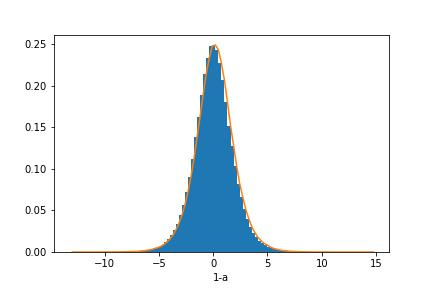
\includegraphics[width=\linewidth]{1-a.jpg}
	\end{figure}
	\newpage
	\item  $F^{-1}(u)=\sqrt{-2\ln(1-u)}$(samples:1000000)
	\begin{figure}[htbp]
		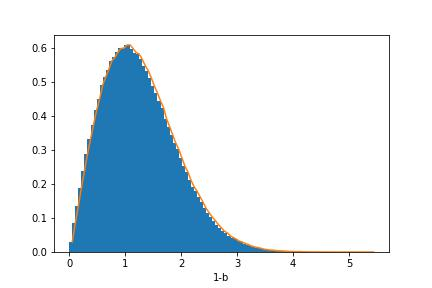
\includegraphics[width=\linewidth]{1-b.jpg}
	\end{figure}
	\newpage
	\item  $F^{-1}(u)= -\ln(1-u)$(samples:1000000)
	
	\begin{figure}[htbp]
		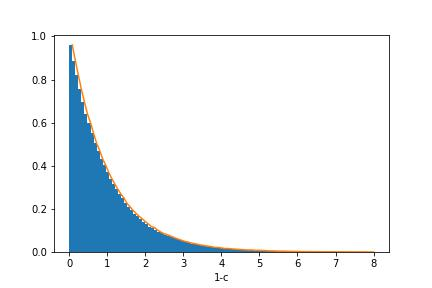
\includegraphics[width=\linewidth]{1-c.jpg}
	\end{figure}
\end{enumerate}
\end{homeworkProblem}
\newpage
% Problem 2
\begin{homeworkProblem}*{BH CH0 \#2}
\begin{enumerate}[(a)]
	\item I treat it as the trial to toss the coin,using the uniform random variables,larger than 0.5,then is success,otherwise it fails
	\begin{figure}[htbp]
		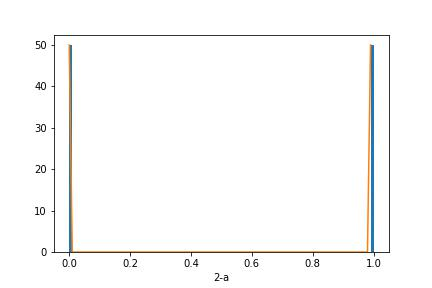
\includegraphics[width=\linewidth]{2-a.jpg}
	\end{figure}
	\newpage
	\item I divide this into many bernolli trials,when trials success ,count+1,so i get the X as the number of success
	\begin{figure}[htbp]
		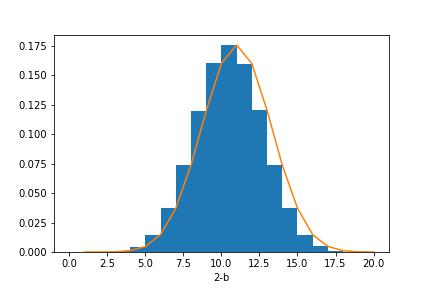
\includegraphics[width=\linewidth]{2-b.jpg}
	\end{figure}
	\newpage
	\item I will treat it as  many bernoli trials,when fail,it will continue,otherwise,record the faiure
	\begin{figure}[htbp]
		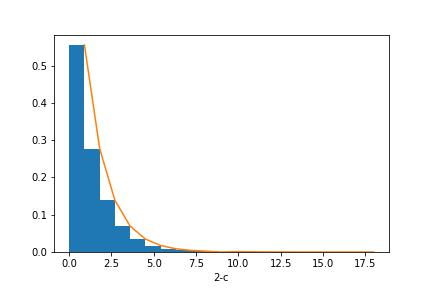
\includegraphics[width=\linewidth]{2-c.jpg}
	\end{figure}
	\newpage
	\item I also treat it as mant bernoli trials,when success equal to 10,I will stop,and record the number of failure
	\begin{figure}[htbp]
		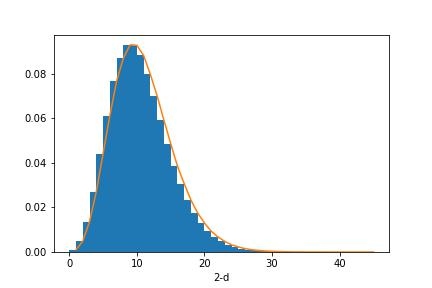
\includegraphics[width=\linewidth]{2-d.jpg}
	\end{figure}
\end{enumerate}


\end{homeworkProblem}


\begin{homeworkProblem}*{BH CH0 \#3}6
	I do the trials by every time multiple a new random variable,if it doesn't satify the condition,then break,count how many variables it multiple,and record count=0,count=1,count=2 to calculate
	\begin{enumerate}[(a)]
		\item I calculate mean by adding total and divide sample number then I can get E(N)=1.0042
		\item I calculate it by adding the sum of squares of (N-E(N)),then divide by sample number I get Var(N)=0.9928
		\item $P(N=0)=0.3614,P(N=1)=0.3752,P(N=3)=0.185$
		\item since the mean and var is same,we can get N$\sim Pois(1)$
	\end{enumerate}
\end{homeworkProblem}

\begin{homeworkProblem}*{BH CH0 \#4}
	\begin{enumerate}
		\item in the sample(1000000),if you switch ,you will win 666058 times,if you don't switch you will win 333942 times,so switch better
		\item in the sample(1000000),when n=4,if you choose strategy 1,you will win 24950($\approx\frac{1}{4}$),if you choose strategy 2,you will win 62481($\frac{2}{3}$ wins),if you choose strategy 3,you will win 75050 times($\frac{3}{4}$ wins),so strategy 3 are best,then 2,then 1, when n=100,samples=100000,strategy 3 is best(98953(0.98953 possibility win)),then strategy 2(63020(0.63020 win)),then strategy 1(1047(0.01047 possibility win))
	\end{enumerate}
\end{homeworkProblem}

\begin{homeworkProblem}*{BH CH0 \#5}
	I perform the simulation,initially set the grid $n\times n$
	by randomly set an unopened site as opened(labeled as one),and check if there 
	is a path from top to bottom(using the depth first search) ,if there exist ,
	record the number of opened sites,and add to the total count,finally divide by samplenumber and calculate the p
	\begin{enumerate}
\item when n=20,I can get the p$\approx 0.5935$
\item when n=50,I can get the p$\approx 0.5928$
\item when n=100,I can get the p $\approx 0.594$
	\end{enumerate}
\end{homeworkProblem}

\end{document}
